

%\documentclass[aip,graphicx]{revtex4-1}
\documentclass[aip,jap, amsmath,amssymb,reprint]{revtex4-1}

\usepackage{graphicx}% Include figure files
\usepackage{dcolumn}% Align table columns on decimal point
\usepackage{bm}% bold math
%\usepackage[mathlines]{lineno}% Enable numbering of text and display math
%\linenumbers\relax % Commence numbering lines
%\draft % marks overfull lines with a black rule on the right
\usepackage{multirow}

\begin{document}

\preprint{AIP/123-QED}

\title{Irradiation influence on  acousto--defect interaction in silicon $n^+$-$p$--structure}
\author{O.~Ya. Olikh}
\email{olikh@univ.kiev.ua}


\author{A.~M. Gorb}


\author{R.~G. Chupryna}

\author{O.~V. Pristay--Fenenkov}%


\affiliation{Faculty of Physics, Taras Shevchenko National University of Kyiv, Kyiv 01601, Ukraine}%Lines break automatically or can be forced with \\



\date{\today}

\begin{abstract}
Abstract. Abstract. Abstract. Abstract.
Abstract.
Abstract. Abstract. Abstract. Abstract. Abstract. Abstract. Abstract.
Abstract. Abstract. Abstract. Abstract. Abstract.
Abstract. Abstract. Abstract. Abstract. Abstract.
Abstract. Abstract. Abstract.
Abstract. Abstract. Abstract. Abstract.
Abstract. Abstract. Abstract. Abstract. Abstract.
Abstract. Abstract. Abstract.
Abstract. Abstract. Abstract.
Abstract. Abstract. Abstract. Abstract.
Abstract.
The
effects of 75 MeV boron (B5+
) ions and 60
Co gamma radiation on the I–V, C–V and spectral responses of
PIN photodiodes were studied systematically to understand the radiation tolerance of the devices.
\end{abstract}

%\pacs{73.30.+y}
\keywords{acousto--defect interaction, silicon, irradiation}

\maketitle %\maketitle must follow title, authors, abstract and \pacs

\section{Introduction}
It has been shown experimentally that ultrasound (US) can effectively interact with defects.
US as defect engineering tool has some advantages:
(i)~locality of the action due to the predominant absorption in regions of deviation in the lattice periodicity;
(ii)~selectivity of the influence, which is achieved by variation of ultrasonic wave (USW) polarization and type;
(iii)~possibility of resonance transformations in the defect system due to the oscillation nature of process action.
(iv)~capability of reversible effect, which is observed in the low intensity USW utilization case.

In the case of piezoelectric semiconductors, the acousto--defect interaction (ADI) is determined mainly by electric field, which accompanies the vibration wave propagation.
This effect is expected and is something related to acousto--electric phenomena.
But US influence on defect system is also observed in non--piezoelectric crystals like silicon, which is dominant material in microelectronic.
Thus it is experimentally observed in silicon crystals and silicon based structures, that US
caused an atomic diffusion \cite{Roman:2010JAP,Roman:2007APL},
transformed a native and an impurity defect \cite{Ostapenko1994,Korotchenkov1995,Olikh2009Sem,Ostapenko1995,Ostrovskii2001}
modified  interior surface states \cite{UST:Medvid,Zaver:2008,Mirsagatov},
created new defect \cite{Savkina2015,Virot}.
Defects are known to determine a most of semiconductor device properties.
And exactly the ADI is a reason of US induced variation of tunneling \cite{Olikh2016JSem,Olikh2011Sem}, a generation--recombination \cite{Davletova2009,Davletova2008,YOlikh2005} and  a thermionic emission \cite{OlikhJAP,Olikh:Ultras} current in silicon barrier structures.

The main mechanisms of elastic vibration--defect interaction in non-piezoelectric crystals are considered to be
the  change  of  population  of  impurity  oscillator  levels  \cite{Pavlovich},
the displacement of impurity atoms with respect to their surroundings \cite{Korotchenkov1995,MirzadeJAP2011,PeleshchakUJF2016},
the decreasing of the diffusion activation  energy \cite{Krevchik},
the local temperature increase by clusters of point defects \cite{MirzadeJAP2005},
the dislocation absorption of ultrasound \cite{Davletova2008,OstrovKor92,Olikh:Ultras2016}.
However to the best of our knowledge, the complete ADI theory in silicon is absent.
One of a top--ranked cause of  this situation is a lack of experimental works, which have focused on investigation of acoustically induced (AI) effects.

Not all silicon defects are acoustically active and are subjected to modification under US action.
The ADI efficiency depends on the defects centers type and structure \cite{UST:Medvid}.
Thus, for example according to \cite{MirzadeJAP2011,PeleshchakUJF2016}, the force acting on the point defect during US loading (USL) is proportionate to volume elastic strain caused by the relaxation of the defect volume $\Delta\Omega_d$.
The irradiation is most widespread and studied methods of alteration of semiconductor defects.
On the one hand, it is shown \cite{YOlikh2007TPL,Parchinskii2006,Gorb2010,Podolian2012}, that high--power US treatment leads to residual changes of the irradiated silicon structure properties.
This effect deals with AI annealing of radiation defects (RDs).
On the other hand, irradiation can be a reason of reversible AI phenomenon initiation \cite{YOlikh2006TPL,YOlikhTPL2011}, which is caused by formation of acoustically active RDs.
Unfortunately, there have only few reports on acoustically driven phenomenon in irradiated silicon structures.


Our goal is to investigate experimentally the AI variations of electrical characteristic which take place in non--irradiated and irradiated $n^+$-$p$--Si structures.
Irradiation was carried by reactor neutrons and a $^{60}$Co--gamma source.
It is expected that $\gamma$--radiation introduces vacancy--impurity point defects (VO$_i$ complex predominantly) \cite{NIEL:Jafari,Gamma:Prabhakara,NIEL:Moll}
whereas neutrons create cluster defects \cite{Rew:Srour,Pintilie}, disordered regions \cite{Neutron:Arutyunov} and C$_i$O$_i$ complex  \cite{NIEL:Moll,neutron:Londos} mainly.
This work represents distinctions of AI changes in silicon structures with different RDs.
The used US intensity was not very high ($<0.5$~W/cm$^2$) to avoid the irreversible defect subsystem modification, which can be deals with a new defect creation, a RDs annealing or a long distance (a great many interatomic distance) AI diffusion.
As a result, the full recovery of $n^+$-$p$--Si structure characteristics was observed after the stop of an AW propagation.
The models of coupled defect level recombination \cite{CDLR:JAP1995,CDLR:JAP}, Shockley--Read--Hall (SRH) recombination, and dislocation--induced impedance \cite{Rsh:Gopal2003,Rsh:Gopal2004} were used to describe the processes in the space charge region,  in the diode base, and shunt resistance respectively.
The interaction of defects with an inhomogeneous USW strain field \cite{MirzadeJAP2011,PeleshchakUJF2016} was recruited to explain the observed AI phenomena.
The investigation would provide not only better ADI understanding but could also facilitate the development of acoustically controlled devices or radiation sensors.



\section{Experimental and calculation details}

The 2 inch (300~$\mu$m thick) p--type boron doped, $<$111$>$ orientation, Czochralski (Cz) silicon wafer having resistivity of 10~$\Omega\cdot$cm was used for fabrication of  $n^+$-$p$--Si structure.
The n$^+$ emitter with carrier concentration of about $10^{19}$~cm$^{-3}$ and thickness of 0.5~$\mu$m was formed by phosphorus implantation.
Then wafer surface was passivated by Al$_2$O$_3$ film and further capped by TiO$_x$ as antireflective coating.
Finally the aluminium front (metal grid) and rear (solid contact) electrodes were deposited by screen printing before rapid annealing.
The samples with area of about $2$~cm$^{2}$ used in experiments were cut from the central part of the wafer.
1 sample  was  irradiated  with  neutrons  in  the fluence  of $\Psi_n=4\cdot10^{11}$~n/cm$^2$  and was denoted as nSC.
2 samples were irradiated  with  $^{60}$Co $\gamma$--rays in the  dose  $D_{\gamma1}=10^6$~rad and $D_{\gamma2}=10^7$~rad and were denoted as g6SC and g7SC respectively.
The label iSC was used for non--irradiated sample.
To avoid an impact of  long--term annealing, which are typical to neutron damaged structure especially \cite{NIEL:Moll,Rew:Srour}, irradiated samples were stored  for  5 years  at  room  temperature before measuring.
According to data \cite{NIEL:Akkerman,Brauning} the neutron dose and gamma fluences can be calculated as $D_n=4.5\cdot10^3$~rad and $\Psi_{\gamma1}=1.6\cdot10^{15}$~$\gamma$/cm$^2$ and $\Psi_{\gamma2}=1.6\cdot10^{16}$~$\gamma$/cm$^2$ respectively.
The non--ionizing energy losses (NIEL) and lifetime damage--constants ($K_\tau$) for neutron
differ from $\gamma$--$^{60}$Co ones by four order of magnitude \cite{NIEL:Akkerman,NIEL:Jafari}:
NIEL$_n=2.04\cdot10^{-3}$~MeV~cm$^2$/g, NIEL$_\gamma=1.07\cdot10^{-7}$~MeV~cm$^2$/g, $K_{\tau,n}=10^{-7}$~cm$^2$/s, $K_{\tau,\gamma}=5\cdot10^{-12}$~cm$^2$/s.
As $(\Psi_{\gamma1}\cdot K_{\tau,\gamma})<(\Psi_{n}\cdot K_{\tau,n})<(\Psi_{\gamma2}\cdot K_{\tau,\gamma})$,
neutrons and $\gamma$-rays are expected to produce a similar damage.


The dark forward current--voltage ($I$--$V$) characteristics of the samples both with and without USL were measured over a temperature range 290--340~K.
The temperature was controlled by differential copper--constantan thermocouple.
Some curves are shown in Fig.~\ref{figIV}.


\begin{figure*}
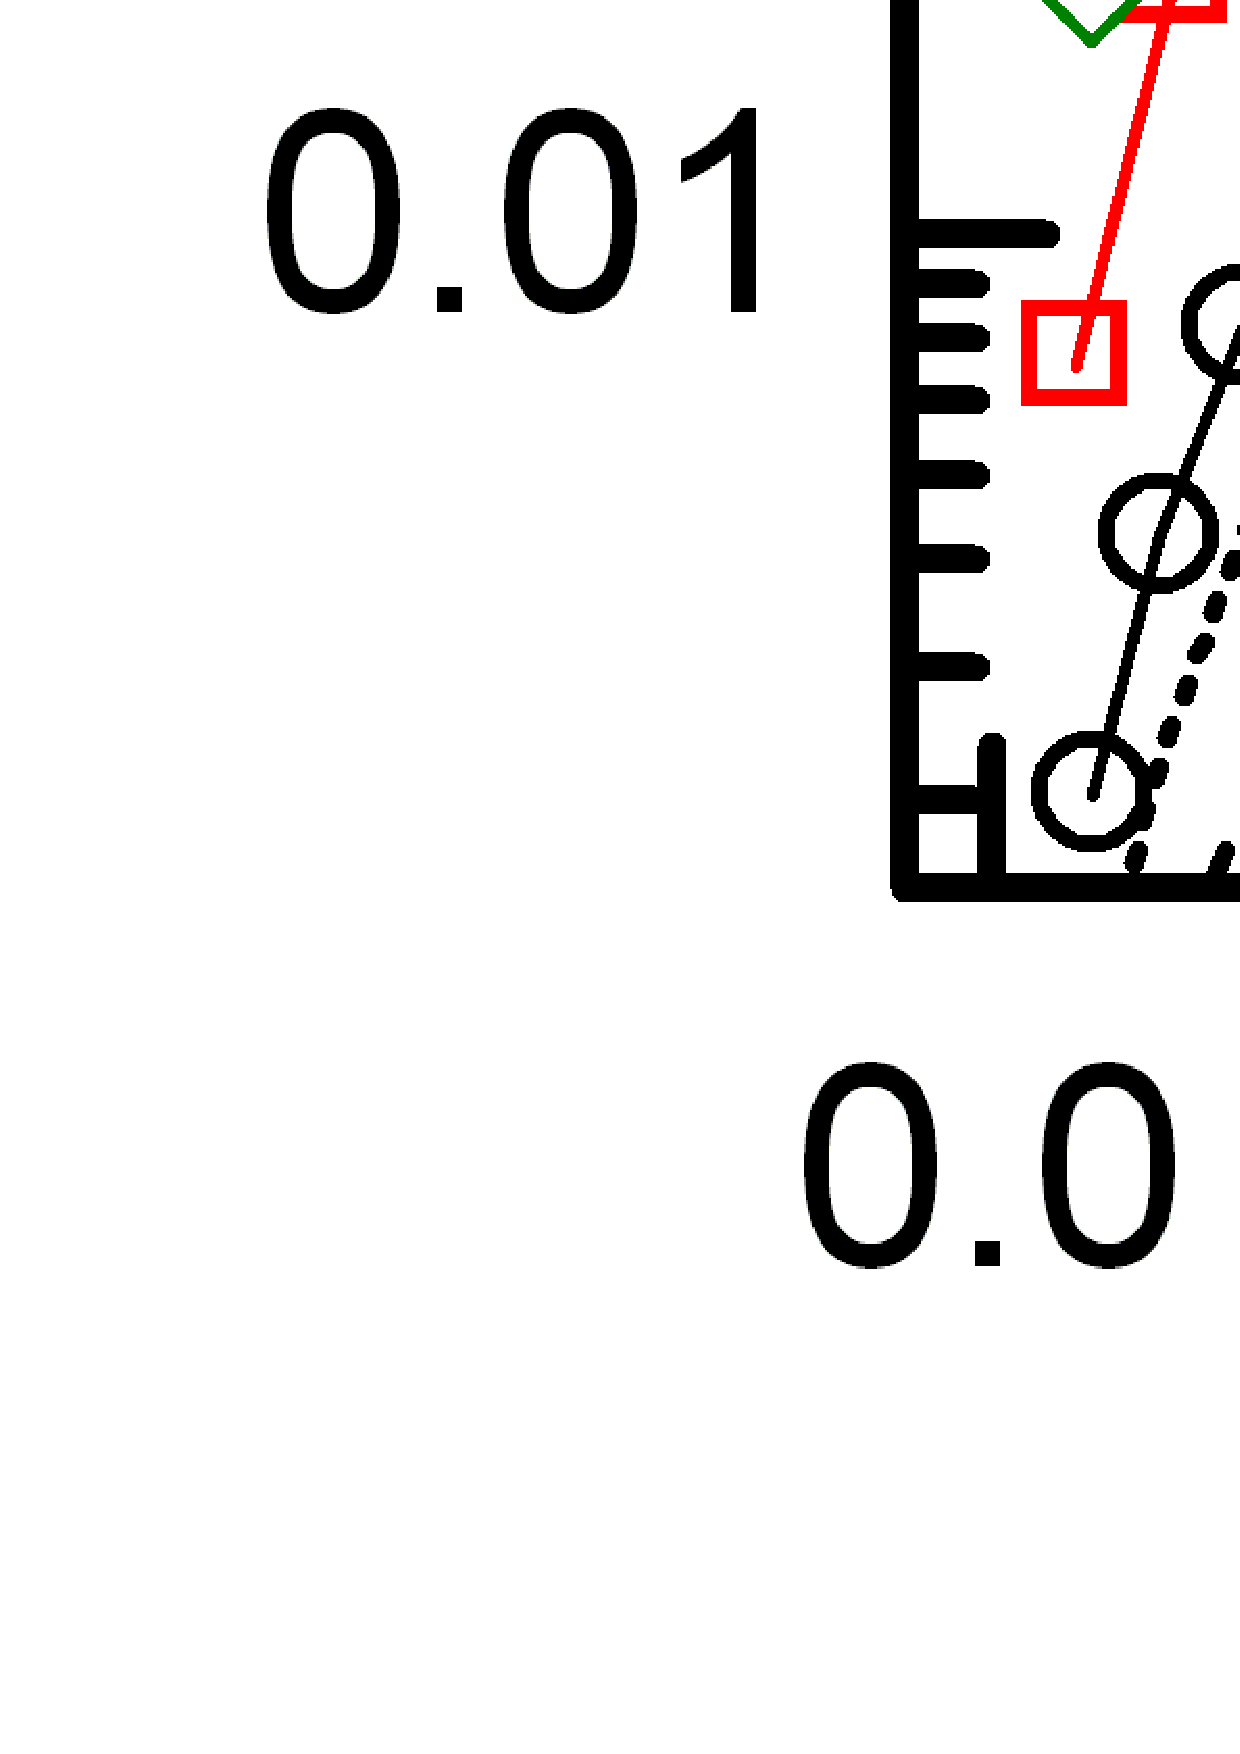
\includegraphics[width=0.7\textwidth]{olikhFig1}%
\caption{\label{figIV}
Dark $I$--$V$ characteristics measured (a) at 306~K for non--irradiated (circles), neutron--irradiated (squares) and gamma--irradiated (diamonds and triangles) structures without USL;
(b) at 301~K (circles) and 341~K (asterisks) with (filled marks, Ui--2) and without (open marks) USL for the iSC.
The marks are the experimental results, the solid lines are the fitted curves using Eqs.~(\ref{eqIV})--(\ref{eqW}).
The dashed, dot--dashed and dotted lines in (a) are the base, SCR and shunt components of iSC current, respectively.
}%
\end{figure*}

The double--diode model of n$^+$--p structure $I$--$V$ characteristics expressed in the following form:
\begin{eqnarray}
I(V,T)&=&I_{SCR}+I_{base}+I_{sh}\;,\label{eqIV}\\
I_{SCR}&=&\frac{qAn_id}{2\tau_{g}}\left\{\exp \left[\frac{q(V-IR_s)}{n_{\mathrm{id}}kT}\right]-1\right\}\,,\label{eqIscr}\\
I_{base}&=&\frac{qAn_i^2}{p_p}\sqrt{\frac{\mu_nkT}{\tau_n}}\left\{\exp \left[\frac{q(V-IR_s)}{kT}\right]-1\right\},\label{eqIbase}\\
I_{sh}&=&(V-IR_s)/R_{sh}\,,\label{eqIsh}
\end{eqnarray}
where
$I_{SCR}$ reflects the overall recombination in the space charge region (SCR),
$I_{base}$ is closely related to recombination in the quasi-neutral region,
$I_{sh}$ is the shunt current,
$A$ is the sample area,
$n_i$ is the intrinsic carrier concentration,
$\tau_{g}$ is the SCR carrier lifetime,
$d$ is the  SCR thickness:
\begin{equation}
\label{eqW}
    d=\sqrt{\frac{2 \varepsilon \varepsilon_0}{q p_p}\left[
     \frac{E_g}{q}-\frac{kT}{q}\ln\!\left(\frac{N_vN_c}{p_pn_n}\right)-\frac{2kT}{q}-V\right]},
\end{equation}
$\varepsilon$ is the permittivity (11.7 for Si),
$p_p$ and $n_n$ are the majority carrier concentration in the $p$-- and $n$--type regions,
$E_g$ is the semiconductor band gap,
$N_c$ and $N_v$ are the effective density of states in the conduction and valence bands;
$n_{\mathrm{id}}$ is the ideality factor of the nonideal current components,
$R_s$ and $R_{sh}$ are the series and shunt resistances of the structure,
$\mu_n$ and $\tau_n$ are the electron (minority carrier) mobility and lifetime in the diode base.


We used Eqs. (\ref{eqIV})--(\ref{eqW}) to fit the experimental data and $\tau_g$, $\tau_n$, $n_{\mathrm{id}}$, $R_{sh}$, and $R_s$ were taken as the  fittings parameters.
The known \cite{ni:Green,Schroder2006,Markvart} temperature dependencies of $n_i$, $E_g$, and $\mu_n$ were used.
The extremely good fit to the experimental data was obtained --- see Fig.~\ref{figIV}.
In particular, the $R_s$ value 1~$\Omega$ was determined for all samples.


In the USL case, the transverse acoustic waves (AWs) with frequency of $4.2$~MHz were exited with help of a piezoelectric transducer and were injected in samples from the base side in the [111]--direction.
The US intensities $W_{\mathtt{US}}$, amplitudes of both lattice deformation $\xi_{\mathtt{US}}$ and lattice atom
displacement  in AW $u_{\mathtt{US}}$ are listed in Table~\ref{tabUSL}.
It was reported previously \cite{Ostapenko1995,Olikh:Ultras,Ostrovskii2001} that a characteristic time of change in the silicon structure parameters under the ultrasound action  did not exceed $2\cdot10^3$~s.
In order to wait till the acoustically induced (AI) transitional period the following experimental procedure has been used.
After USL start the sample was kept at room temperature during 60 min and then the $I$--$V$ measurements and the sample heating were started.
In order to avoid the effect of piezoelectric field on $I$--$V$ characteristics, the piezoelectric transducer has been shielded.


\begin{table}
\caption{\label{tabUSL}The parameters of ultrasound loadings.
}
\begin{ruledtabular}
\begin{tabular}{lcccr}
Sample&$W_{\mathtt{US}}$ (W/cm$^2$)&$\xi_{\mathtt{US}}$ ($10^{-6}$)&$u_{\mathtt{US}}$ (nm)&Label\\
\hline
iSC&0.22&3.1&0.7&Ui--1\\
%\multirow{2}{*}{iSC}&0.22&3.1&0.7&Ui--1\\
&0.40&4.2&0.9&Ui--2\\
nSC&0.21&3.0&0.7&Un--1\\
%\multirow{2}{*}{nSC}&0.21&3.0&0.7&Un--1\\
&0.36&4.1&0.9&Un--2\\
g6SC&0.32&3.7&0.8&Ug6--2\\
g7SC&0.24&3.2&0.7&Ug7--1\\
%\multirow{2}{*}{g7SC}&0.24&3.2&0.7&Ug7--1\\
&0.40&4.2&0.9&Ug7--2\\
\end{tabular}
\end{ruledtabular}
\end{table}


The linear and non-linear fitting were done by using the least-squares and differential evolution \cite{DEWang} method, respectively.


\section{Results and Discussion}
\subsection{Space charge region\label{SCR}}
The $I$--$V$ characteristics parameters, which deal with SCR phenomena, are $n_{\mathrm{id}}$ and $\tau_{g}$.
The finding temperature dependences of ideality factor and SCR lifetime are shown in Fig.~\ref{fig_n} and Fig.~\ref{fig_TAUg} respectively.

\begin{figure*}
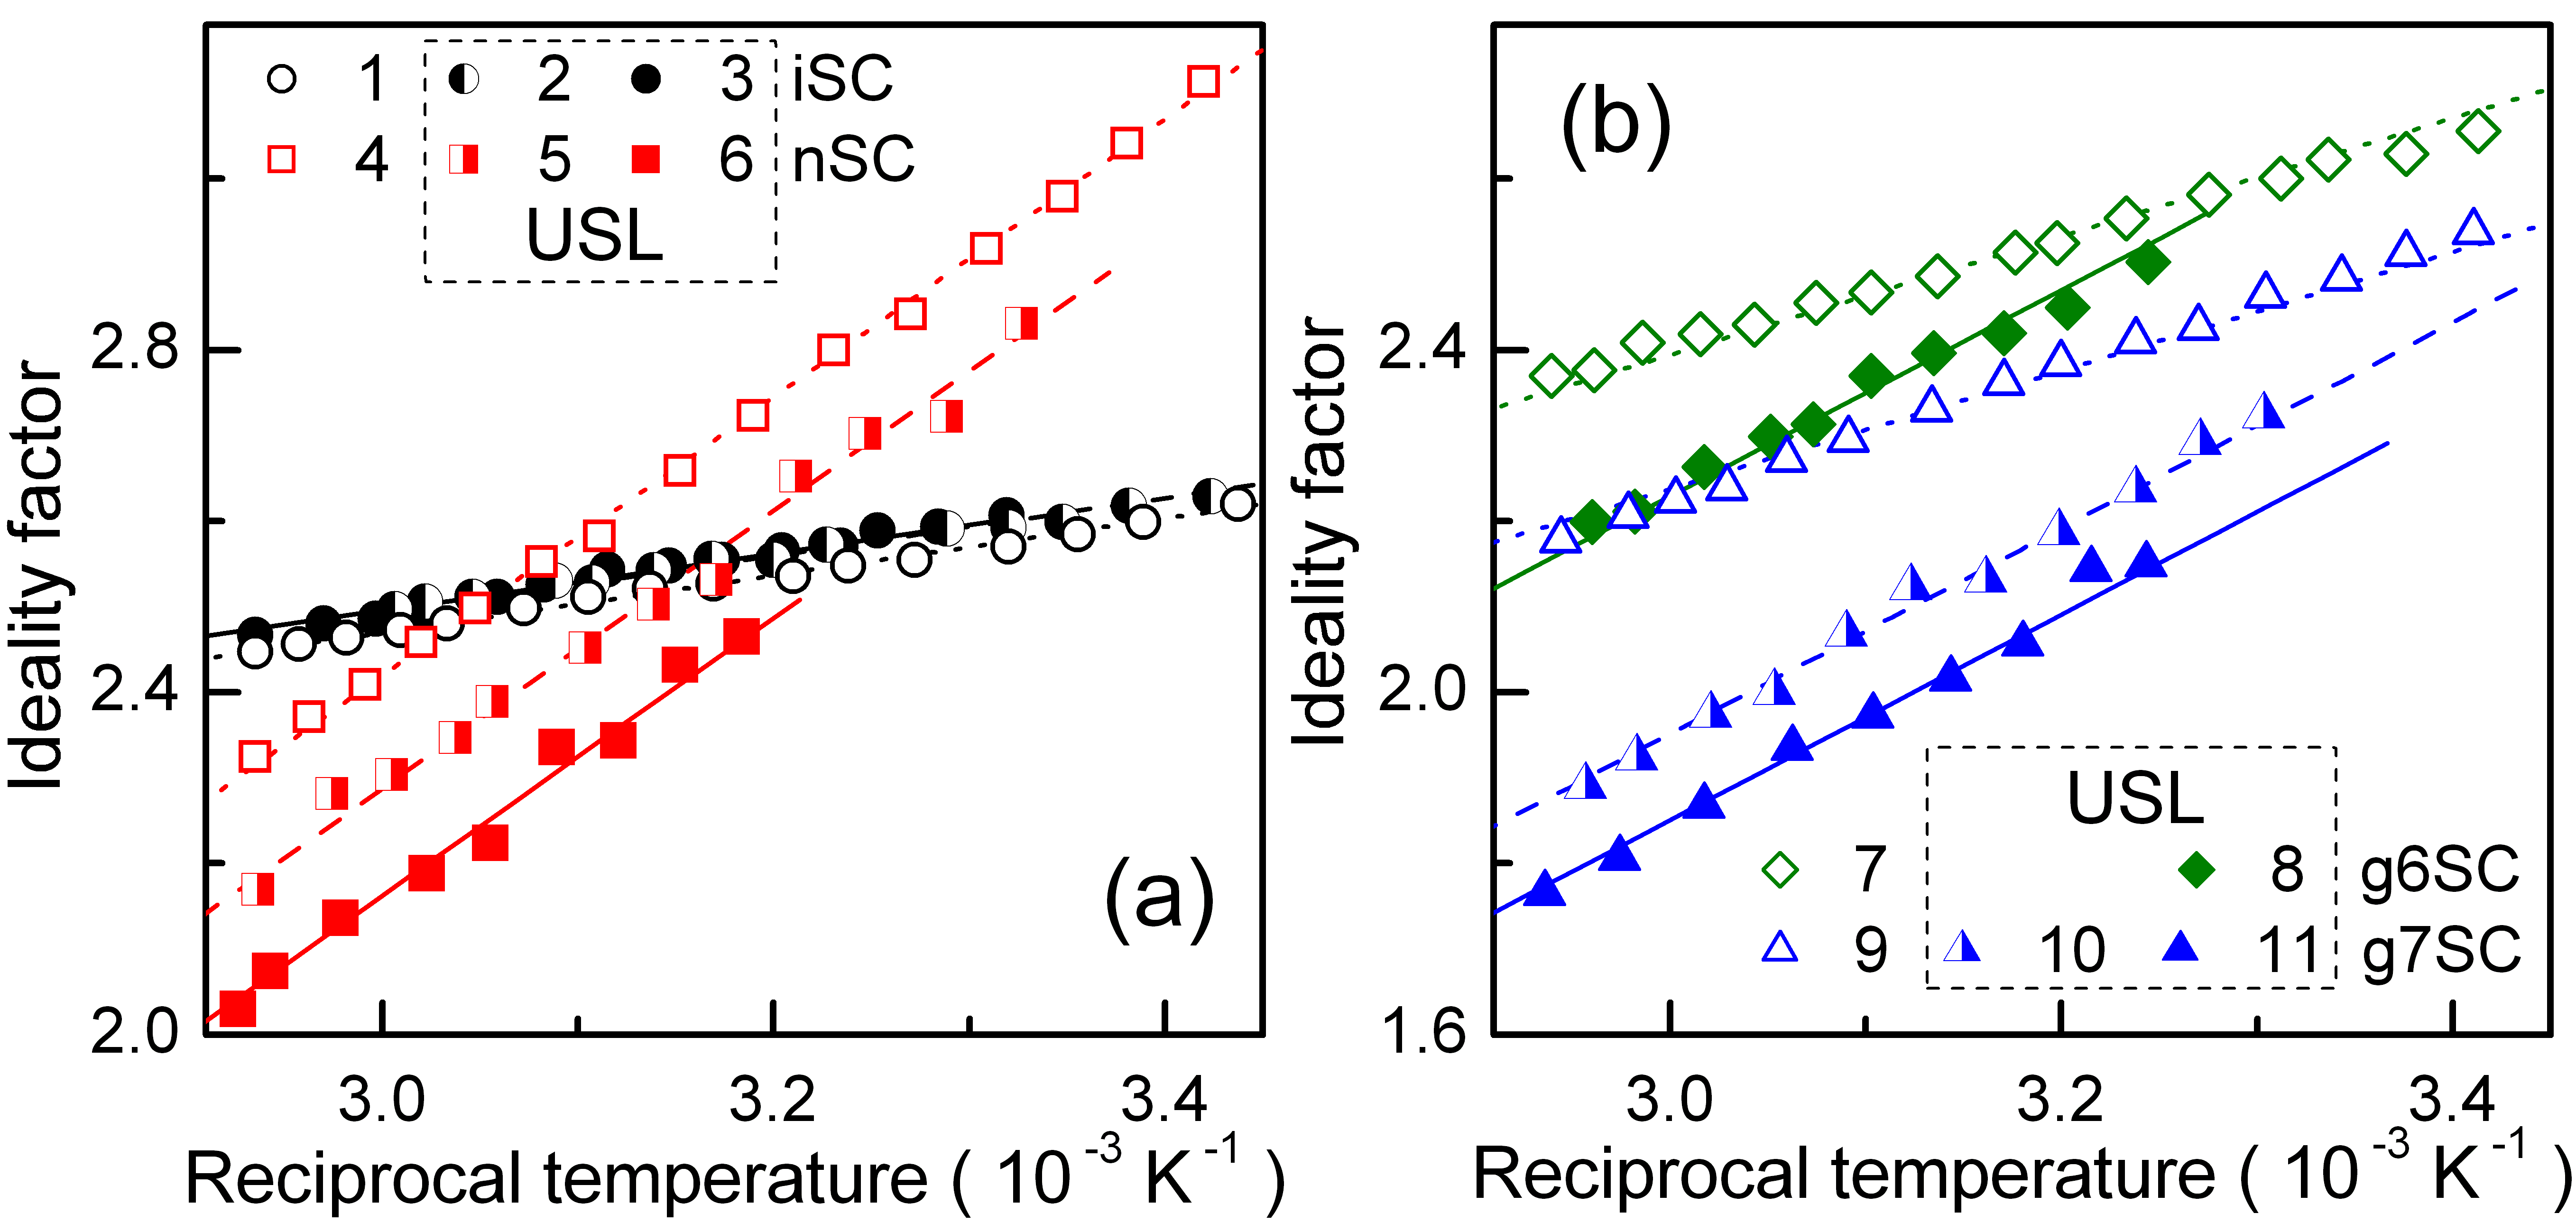
\includegraphics[width=0.7\textwidth]{olikhFig2}%
\caption{\label{fig_n}
Temperature dependences of ideality factor for non--irradiated (curves 1--3, circles),
neutron--irradiated (4--6, squares) and $\gamma$--irradiated (7--11, diamonds and triangles) samples.
The curves 1, 4, 7 and 9 (open marks) are obtained without USL,
curves 2, 3, 5, 6, 8, 10, and 11 correspond to
Ui--1, Ui--2, Un--1, Un--2, Ug6--2, Ug7--1, and Ug7--2 respectively.
The marks are the experimental results, the lines are the fitted curves using Eq.~(\ref{eq_nT}).
}%
\end{figure*}

\begin{figure*}
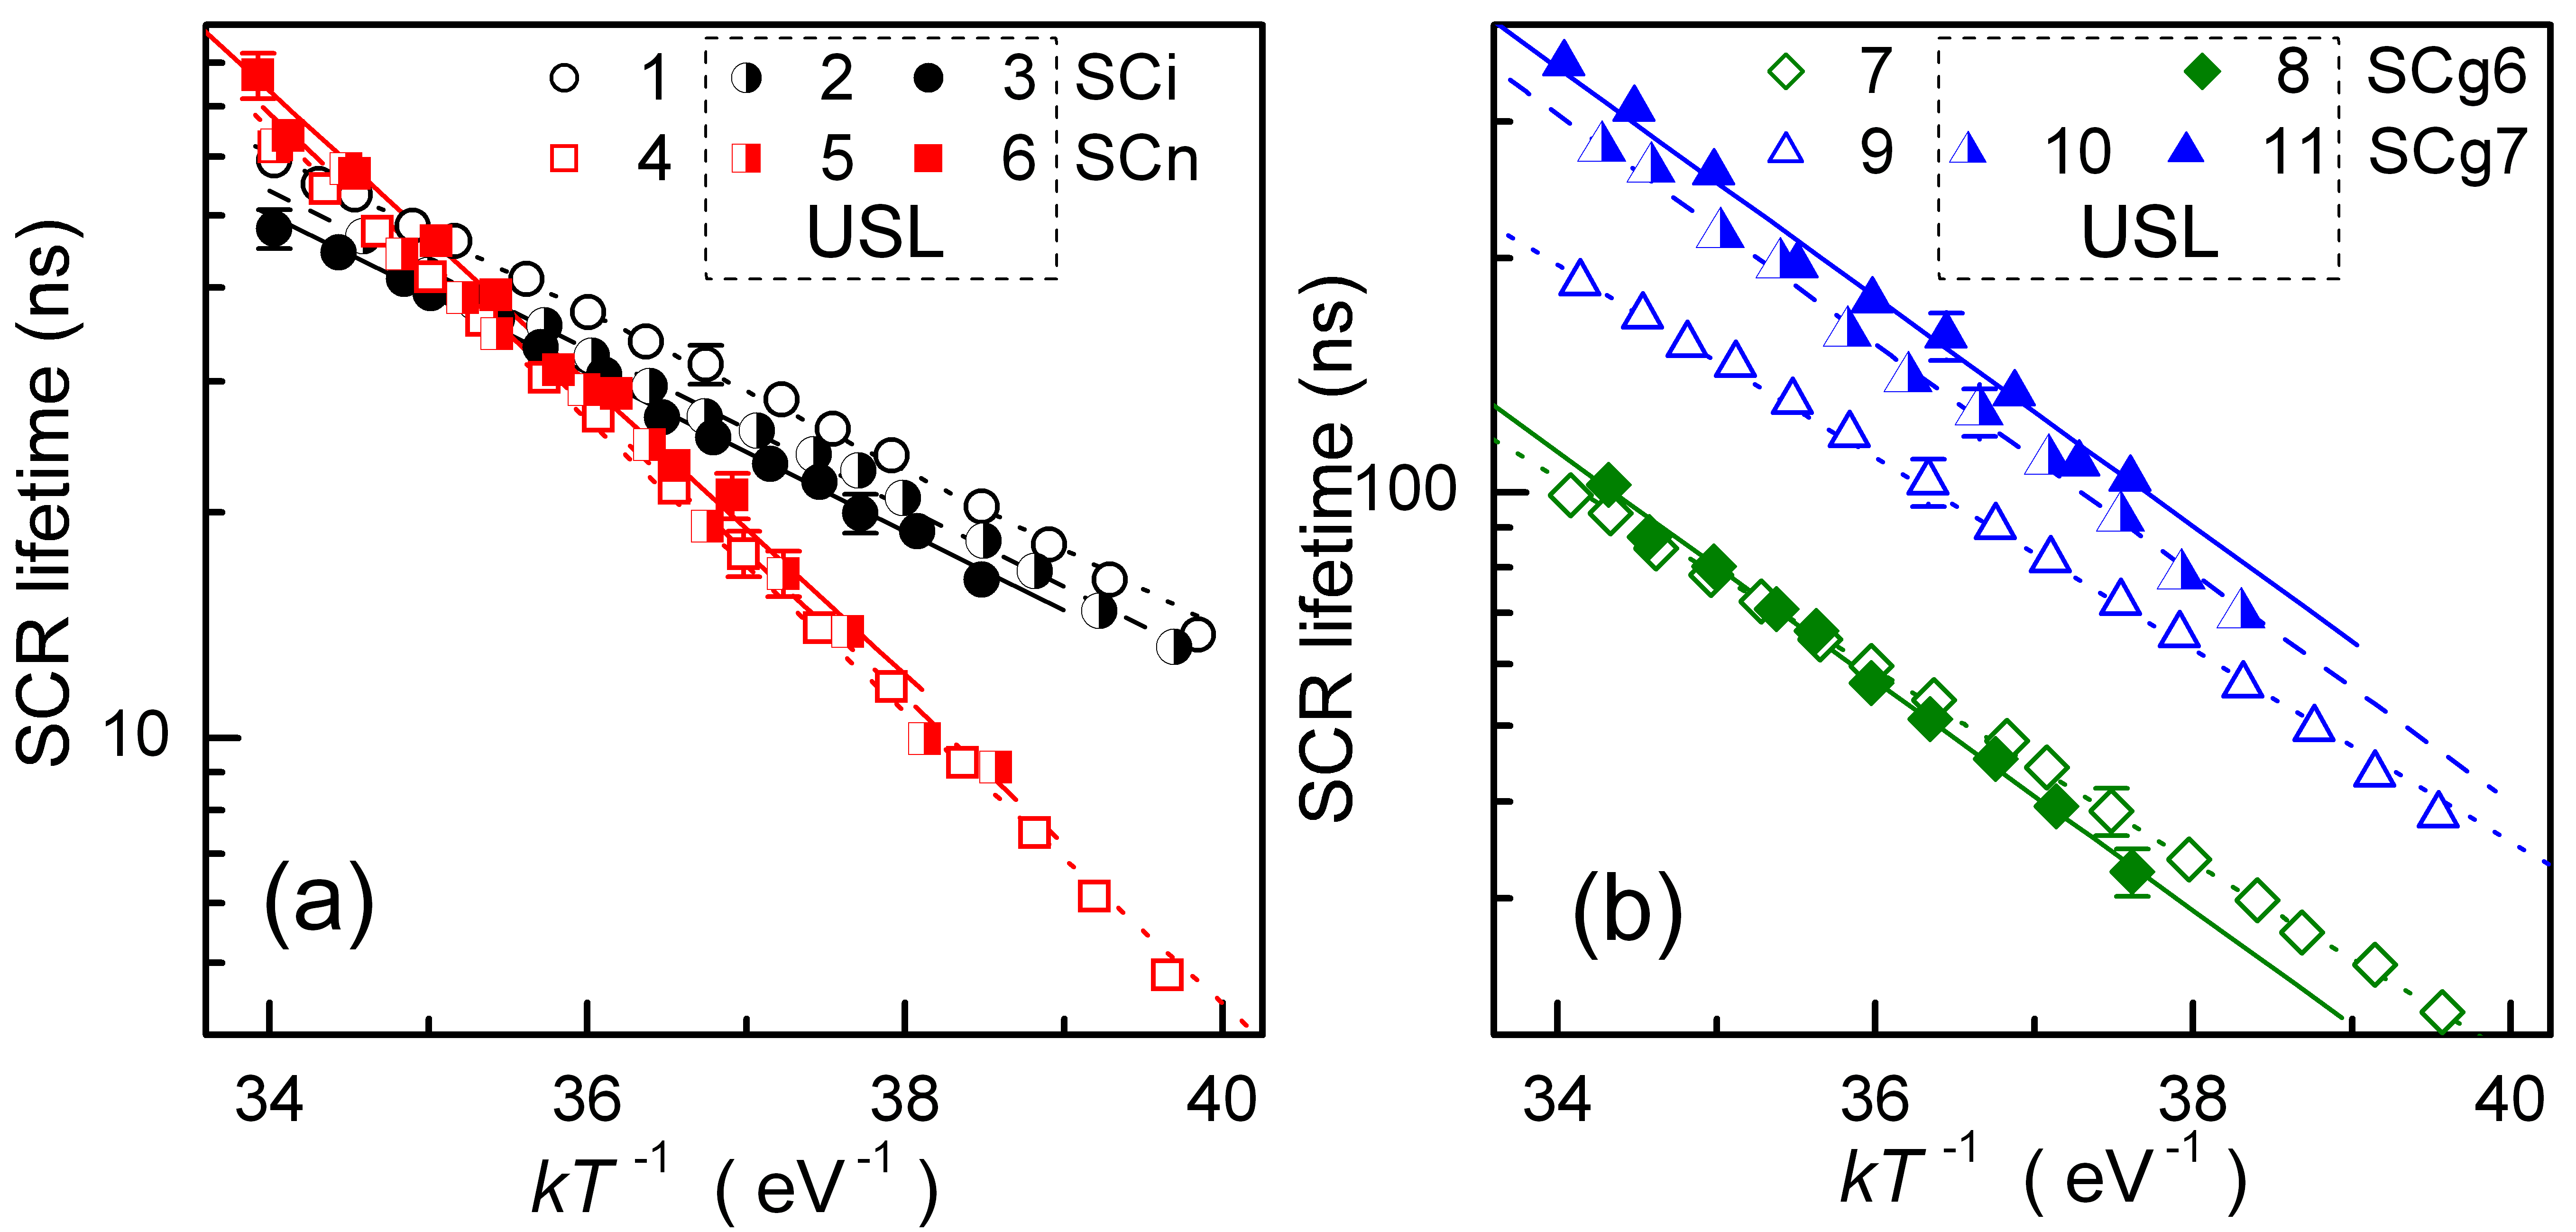
\includegraphics[width=0.7\textwidth]{olikhFig3}%
\caption{\label{fig_TAUg}
Temperature dependences of SCR lifetime for non--irradiated (curves 1--3, circles),
neutron--irradiated (4--6, squares) and $\gamma$--irradiated (7--11, diamonds and triangles) samples.
The curves 1, 4, 7 and 9 (open marks) are obtained without USL,
curves 2, 3, 5, 6, 8, 10, and 11 correspond to
Ui--1, Ui--2, Un--1, Un--2, Ug6--2, Ug7--1, and Ug7--2 respectively.
The marks are the experimental results, the lines are the fitted curves using Eq.~(\ref{eq_TAUgT}).
}%
\end{figure*}

As one can recognize, ideality factor decreases with temperature increase and plots $n_{\mathrm{id}}$ vs $1/T$  are close to linear.
Thus dependence $n_{\mathrm{id}}(T)$ can be expressed as
\begin{equation}
\label{eq_nT}
    n_{\mathrm{id}}(T)=n_{\mathrm{id},\infty}+T_{\mathrm{id}}/T\:.
\end{equation}
On the other hand, the thermoactivated SCR carrier lifetime growth  is observed over the explored temperature range - see Fig.~\ref{fig_TAUg}.
The following equation allows to describe sufficiently $\tau_{g}$ temperature dependence:
\begin{equation}
\label{eq_TAUgT}
    \tau_{g}(T)=\tau_{g0}\exp\left(-\frac{E_{\tau g}}{kT}\right)\:.
\end{equation}
The $T_{\mathrm{id}}$ and $E_{\tau g}$ values, which were determined for both non-irradiated and irradiated samples with as well as without USL are listed in Table~\ref{tabTpar}.

\begin{table}
\caption{\label{tabTpar}Characteristics of temperature dependences of $n^+$-$p$--Si structure parameters.
}
\begin{ruledtabular}
\begin{tabular}{lccc}
Sample&USL&$T_{\mathrm{id}}$ (K)&$E_{\tau g}$ (eV)\\
\hline
\multirow{3}{*}{iSC}&non&$330\pm30$&$0.24\pm0.01$\\
&Ui--1&$310\pm30$&$0.24\pm0.01$\\
&Ui--2&$360\pm30$&$0.24\pm0.01$\\
\multirow{3}{*}{nSC}&non&$1610\pm70$&$0.45\pm0.02$\\
&Un--1&$1600\pm70$&$0.44\pm0.02$\\
&Un--2&$1680\pm70$&$0.44\pm0.02$\\
\multirow{2}{*}{g6SC}&non&$610\pm40$&$0.28\pm0.01$\\
&Ug6--2&$1080\pm50$&$0.33\pm0.02$\\
\multirow{3}{*}{g7SC}&non&$770\pm50$&$0.29\pm0.01$\\
&Ug7--1&$1260\pm60$&$0.34\pm0.02$\\
&Ug7--2&$1270\pm60$&$0.35\pm0.02$\\
\end{tabular}
\end{ruledtabular}
\end{table}

We want to stress, that

\noindent
(i)~irradiation leads to $T_{\mathrm{id}}$ and $E_{\tau g}$ changes, the g6SC's ideality factor characteristic temperature and SCR lifetime characteristic energy values are closely related to g7SC ones at similar conditions;

\noindent
(ii)~USL affects $n_{\mathrm{id}}$ and $\tau_g$ values, absolute AI changes of ideality factor $\Delta n_{\mathrm{id}}=n_{\mathrm{id},\mathtt{US}}-n_{\mathrm{id},in}$ and
relative AI changes of SCR lifetime $\varepsilon_{\tau g}=(\tau_{g,\mathtt{US}}-\tau_{g,in})/\tau_{g,in}$
(where subscripts ``$\mathtt{US}$'' and ``$in$'' identify with values,
%$n_{\mathtt{US}}(T)$ and $n_{in}(T)$ are the ideality factor,
which obtained at the same temperature with and without USL respectively)
are listed in Table~\ref{tabAIchange};

\noindent
(iii)~$\Delta n_{\mathrm{id}}$ and $\varepsilon_{\tau g}$ vary with $W_{\mathtt{US}}$ enhancement, whereas $T_{\mathrm{id}}$ and $E_{\tau g}$ values do not depend on ultrasound intensity practically.


\noindent
(iv)~USL results in both $T_{\mathrm{id}}$ and $E_{\tau g}$ increase in $\gamma$--irradiated samples --- see Fig.~\ref{fig_n}(b) and Fig.~\ref{fig_TAUg}(b), but same effect is not observed in non--irradiated and neutron--irradiated samples --- see Fig.~\ref{fig_n}(a) and Fig.~\ref{fig_TAUg}(a);

\noindent
(v)~$\Delta n_{\mathrm{id}}$ and $\varepsilon_{\tau g}$ have an opposite sign for non--irradiated and irradiated samples
(for SCg6 not in whole temperature range);

\noindent
(vi)~ideality factor is varied by USL more effectively in irradiated samples;


%\noindent
%(vii)~US influence efficiency for $\gamma$--irradiated samples rises with dose;




\begin{table}
\caption{\label{tabAIchange}Acoustically induced change of $n^+$-$p$--Si structure parameters (at 330~K).
}
\begin{ruledtabular}
\begin{tabular}{lccccc}
Sample&USL&$\Delta n_{\mathrm{id}}$ &$\varepsilon_{\tau g}$ &$\varepsilon_{\tau r}$ &$\varepsilon_{Rsh}$ \\
&&\mbox{($\pm0.01$)}&($\pm5$\%)&($\pm12$\%)&($\pm5$\%)\\
\hline
\multirow{2}{*}{iSC}&Ui--1&0.02&-14&-43&-15\\
&Ui--2&0.03&-17&-58&-32\\
\multirow{2}{*}{nSC}&Un--1&-0.13&5&-60&-19\\
&Un--2&-0.26&13&-75&-34\\
g6SC&Ug6--2&-0.15&2&-67&-3\\
\multirow{2}{*}{g7SC}&Ug7--1&-0.26&49&-39&-5\\
&Ug7--2&-0.36&70&-58&-8\\
\end{tabular}
\end{ruledtabular}
\end{table}


For purpose of the present consideration, it is important to discuss an recombination mechanism in the SCR of the investigated samples.
According to classical SRH theory, an ideality factor must be less than 2 and
$\tau_g$ temperature dependence is expected \cite{TAUg:Schroder,TAUg:Aharoni} to be described by the relation  $\tau_g\simeq2\tau_n\sqrt{\sigma_n/\sigma_p}\cosh\left[\left(E_t-E_i\right)/kT\right]$
(where $\sigma_n$, $\sigma_p$, and  $E_t$ are the electron and hole capture cross sections (CCSs) and the energy  level of  the  recombination  center,
$E_i$  is the  intrinsic  energy level).
In the our case, $n_{\mathrm{id}}$ is lager than 2 and $\tau_g$ increases with temperature.
Therefore SRH theory is inapplicable to the investigated samples.
Several attempts to explain large $n_{\mathrm{id}}$ have been made with various models \cite{Heide,Beier,Shah,Kaminski_n}.
But all observed features of SCR recombination (ideality factor large value, independence on light intensity, dependence on temperature
as well as carrier lifetime small value and thermoactivated behavior) can be explained by the model of coupled defect level recombination (CDLR) \cite{CDLR:JAP1995,CDLR:JAP} only.
This model provides a rapid  direct  charge  transfer  between  defect levels.
Such phenomenon have been observed experimentally firstly \cite{DAPR:Chen1991,DAPR:Chen1994} and then it was recruited to explain process in semiconductor diodes \cite{CDLR:JAP1995,CDLR:JAP,CDLR:SSP}.

According to the CDLR model, recombination is the result of carrier exchange between two defect level and crystal bands.
In particular, it is proposed \cite{CDLR:JAP} that the recombination rate is dominated by sites where an acceptor--like defect is coupled to a donor-like defect.
In the simplified case, when
no carrier exchange between the donor level $E_t^{\mathtt{D}}$ and the valence band
as well as between the acceptor level $E_t^{\mathtt{A}}$ and the conduction band,
%In the simplified case, when
%carrier exchanges between the donor level and the conduction band,
%between the acceptor level and the valence band,
%and between the donor level and the acceptor level are allowed only,
the recombination rate $R$ can be expressed\cite{CDLR:JAP1995} as
\begin{eqnarray}
R&=&\frac{R_{12}-\sqrt{R_{12}^{\,2}-4\tau_{n}^{\mathtt{D}}\tau_{p}^{\mathtt{A}}(np-n_i^2)(1-\epsilon)}}{2\tau_{n}^{\mathtt{D}}\tau_{p}^{\mathtt{A}}(1-\epsilon)}\;,\label{eqR}\\
R_{12}&=&\frac{(n+n_{\mathtt{D}})(p+p_{\mathtt{A}})}{R_{\mathtt{DA}}}+
\tau_{n}^{\mathtt{D}}(p+p_{\mathtt{D}})+\tau_{p}^{\mathtt{A}}(n+n_{\mathtt{A}}),\label{eqR12}\\
\tau_{n}^{\mathtt{D}}&=&(N_{\mathtt{D}}\,\sigma_{n}^{\mathtt{D}}\,\upsilon_{\mathrm{th},n})^{-1},\,\,\,\,
\tau_{p}^{\mathtt{A}}=(N_{\mathtt{A}}\,\sigma_{p}^{\mathtt{A}}\,\upsilon_{\mathrm{th},p})^{-1},\label{eqTAU}
%\\
%n_{\mathtt{D,A}}&=&N_c(g_0^{\mathtt{D,A}}/g_1^{\mathtt{D,A}})\cdot\exp[-E_t^{\mathtt{D,A}}/kT],\label{eq_nDA}\\
%p_{\,\mathtt{D,A}}&=&N_v(g_1^{\mathtt{D,A}}/g_0^{\mathtt{D,A}})\cdot\exp[-(E_g-E_t^{\mathtt{D,A}})/kT],\label{eq_pDA}\\
%\epsilon&=&(g_1^{\mathtt{D}}\,g_0^{\mathtt{A}})/(g_0^{\mathtt{D}}\,g_1^{\mathtt{A}})\cdot\exp[-(E_t^{\mathtt{A}}-E_t^{\mathtt{D}})/kT]\,,\label{eqEPS}
\end{eqnarray}
where
$R_{\mathtt{DA}}$ is the coupling parameter,
%$n_{\mathtt{D,A}}=N_c\frac{g_0^{\mathtt{D,A}}}{g_1^{\mathtt{D,A}}}\exp\left(\frac{E_c-E_t^{\mathtt{D,A}}}{kT}\right)$
%$\tau_{n,p}^{\mathtt{D,A}}=(N_{\mathtt{DAP}}\sigma_{n,p}^{\mathtt{D,A}}\upsilon_{th,n,p})^{-1}$ ,
%$N_{\mathtt{DAP}}=(N_{\mathtt{D}}+N_{\mathtt{A}})/2$ is the donor--acceptor--pair (DAP) density,
$N_{\mathtt{D}}$ and $N_{\mathtt{A}}$ are the density of the donor and acceptor--like defects,
$\sigma_{n}^{\mathtt{D}}$ and $\sigma_{p}^{\mathtt{A}}$ are electron CCS of donor and hole CCS of acceptor,
$\upsilon_{\mathrm{th},n}$ and $\upsilon_{\mathrm{th},p}$ are the thermal electron and hole velocity,
$n_{\mathtt{D,A}}$, $p_{\,\mathtt{D,A}}$, and $\epsilon$ depend on $E_t^{\mathtt{D}}$, $E_t^{\mathtt{A}}$, and level degeneracy  factors.
%$\epsilon=\frac{g_1^{\mathtt{D}}g_0^{\mathtt{A}}}{g_0^{\mathtt{D}}g_1^{\mathtt{A}}}\exp\left(\frac{E_t^{\mathtt{D}}-E_t^{\mathtt{A}}}{kT}\right)$,
%$E_t^{\mathtt{D}}$ and $E_t^{\mathtt{A}}$ are the donor and acceptor levels  measured  from  the  conduction  band edge,
%$g_{0,1}$ are degeneracy  factors  of  the empty  and occupied  levels.
As $\tau_g\propto R^{-1}$, last ones are expected to provide a thermoactivated SCR lifetime behavior.
Unfortunately, the functional relation between $I$--$V$ characteristic parameters and attributes of defects, which take part in CDLR, is not suggested.

According to Steingrube \emph{et al}.\cite{CDLR:JAP},
SSC for defect in a pair is differs from one for isolated defect and depends on the distance between donor and acceptor $r$:
\begin{equation}
\label{eqSigma}
\sigma_{n,p}^{\mathtt{D,A}}(r)=A_{n,p}^{\mathtt{D,A}}\,r^2\,,
\end{equation}
where $A_{n}^{\mathtt{D}}$ and $A_{p}^{\mathtt{A}}$ are some constant.
Besides, $R_{\mathtt{DA}}$ is proportional to the overlap integral of the wave functions.
If both defects are characterized by H--like radial--symmetric wave function and by equal Bohr radius $a_0$,
the following expression can be used \cite{CDLR:JAP}:
\begin{equation}
\label{eqRda}
R_{\mathtt{DA}} (r) \propto N_{\mathtt{D}}N_{\mathtt{A}}\left[1+\frac{r}{a_0}+\frac{1}{3}\left(\frac{r}{a_0}\right)^2\right]
   e^{-r/a_0}\,.
%   \exp\left(-\frac{r}{a_0}\right)\,.
\end{equation}


%According to Steingrube \emph{et al}.\cite{CDLR:JAP},
%$\sigma_{n}^{\mathtt{D}}$, $\sigma_{p}^{\mathtt{A}}$,  and $R_{\mathtt{DA}}$
%depend on the distance between donor and acceptor $r$.
%If wave functions for both defects are characterized by H--like radial--symmetric and equal Bohr radius $a_0$,
%%In the case of H--like radial--symmetric wave functions for the defects with equal Bohr radii $a_0$,
%the following expression can be used \cite{CDLR:JAP}:
%\begin{eqnarray}
%\sigma_{n,p}^{\mathtt{D,A}}&=& \sigma_{n,p}^{0\mathtt{D,A}}\left(\frac{r}{r_0^{\mathtt{D,A}}}\right)^2\,,\label{eqSigma}\\
%R_{\mathtt{DA}} &=& C_{\mathtt{DA}}N_{\mathtt{D}}N_{\mathtt{A}}\left[1+\frac{r}{a_0}+\frac{1}{3}\left(\frac{r}{a_0}\right)^2\right]
%   \exp\left(-\frac{r}{a_0}\right)\,,\label{eqRda}
%\end{eqnarray}
%where
%$\sigma_{n}^{0\mathtt{D}}$ and $\sigma_{p}^{0\mathtt{A}}$ are CCS of the isolated (non--coupled) donor and acceptor,
%$r_0^{\mathtt{D}}$, $r_0^{\mathtt{A}}$,  and $C_{\mathtt{DA}}$ are some constant.

In our opinion, the observed reversible AI $n_{\mathrm{id}}$ and $\tau_g$ modifications are induced by
donor--acceptor distance alteration in samples under USL.
Really, according to \cite{MirzadeJAP2011,PeleshchakUJF2016}, the force acting on the point defect during USL can be expressed as
\begin{equation}
\label{eqFd}
F_d=K\,\Delta\Omega_d\frac{\partial \xi(z,t)}{\partial z}\,,
\end{equation}
where
$K$ is the bulk elasticity modulus,
$\Delta\Omega_d$ is the crystal volume change per defect,
$\xi$ is the crystal lattice deformation,
and AW propagates along $z$ direction.
$\partial \xi(z,t)/\partial z\propto \xi_{\mathtt{US}}$.
For interstitial atoms and substitutional impurities with the ionic radius exceeding the ionic radius of matrix
atoms, the $\Delta\Omega_d > 0$, whereas,
for vacancies and substitutional impurities with ionic radius smaller than the ionic radius of matrix atoms,
$\Delta\Omega_d < 0$.
Therefore, a point defect vibrates under USL condition and oscillation amplitude and phase are determined by both defect character and acoustic wave intensity.

\begin{figure}
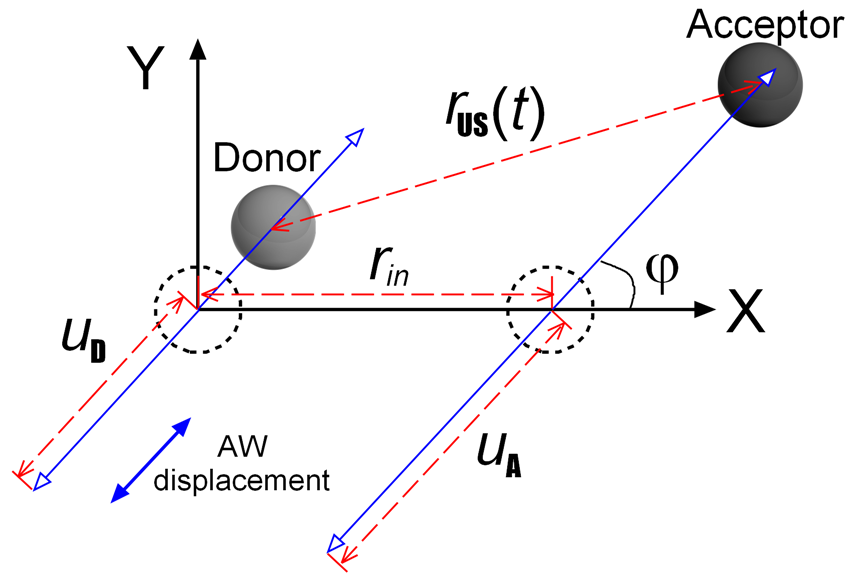
\includegraphics[width=0.45\textwidth]{olikhFig4}%
\caption{\label{fig_Model}
Model of CDLR center behavior under US action.
}%
\end{figure}

Some qualitative conclusion can be drawn from the simplest model, which is shown in Fig.~(\ref{fig_Model}).
Initially donor and acceptor are situated at distance $r_{in}$.
Axis X is drawn through point defect inial positions.
During USL defects would vibrate with amplitudes $u_\mathtt{D}$ and $u_\mathtt{A}$.
Vibration axis coincides with AW displacement direction and forms angle $\varphi$ with  X--axis.
The amplitudes depend on $\xi_{U\!S}$, defect elastic strain ($\Delta\Omega_d^\mathtt{D}$ and $\Delta\Omega_d^\mathtt{A}$), defect coupling  and can be different.
According to suggested model, the donor--acceptor distance in the sample with USL $r_\mathtt{US}$ depends on time $t$:
%\begin{eqnarray}
%\label{eqrUS}
%r_\mathtt{US}(t)&=&\left\{[r_{in}+u_\mathtt{A}\cos(\omega_\mathtt{US}t+\delta)-u_\mathtt{D}\cos(\omega_\mathtt{US}t)]^2\cos^2\varphi \right.\nonumber\\
%   && \left.+ [u_\mathtt{A}\cos(\omega_\mathtt{US}t+\delta)-u_\mathtt{D}\cos(\omega_\mathtt{US}t)]^2\sin^2\varphi\right\}^{0.5}\,,
%\end{eqnarray}
\begin{multline}
\label{eqrUS}
r_\mathtt{US}(t)=\left\{[r_{in}+u_\mathtt{A}\cos(\omega_\mathtt{US}t+\delta)-u_\mathtt{D}\cos(\omega_\mathtt{US}t)]^2\cos^2\varphi \right.\\
    \left.+ [u_\mathtt{A}\cos(\omega_\mathtt{US}t+\delta)-u_\mathtt{D}\cos(\omega_\mathtt{US}t)]^2\sin^2\varphi\right\}^{0.5}\,,
\end{multline}
where $\omega_\mathtt{US}$ is the US cyclic frequency,
$\delta$ is the phase shift between donor and acceptor vibration.

We use Eqs.~(\ref{eqSigma})--(\ref{eqRda}) to estimate AI relative changes of CCS
$\varepsilon_\sigma=[\sigma_{\mathtt{US}}-\sigma(r_{in})]/\sigma(r_{in})$
and coupling parameters $\varepsilon_{\mathtt{RDA}}=[R_{\mathtt{DA,US}}-R_\mathtt{DA}(r_{in})]/R_\mathtt{DA}(r_{in})$,
where $\sigma_{\mathtt{US}}$ and $R_{\mathtt{DA,US}}$ are averaged over the AW period $T_\mathtt{US}$:
\begin{equation*}
\label{eqAver}
\sigma_{\mathtt{US}}=\frac{1}{T_\mathtt{US}}\int^{T_\mathtt{US}}_0\!\!\!\!\!\!\sigma(r_\mathtt{US}(t))dt\,,
R_{\mathtt{DA,US}}=\frac{1}{T_\mathtt{US}}\int^{T_\mathtt{US}}_0\!\!\!\!\!\!R_{\mathtt{DA}}(r_\mathtt{US}(t))dt\,.
\end{equation*}
While estimating, relaxation time in the CDLR sub--system is assumed to be considerably less than $T_\mathtt{US}$
and the previously used\cite{CDLR:JAP} value $a_0=3.23$~nm is utilized.
Besides, the chosen $u_\mathtt{D}$ and $u_\mathtt{A}$ values are commensurate with $u_\mathtt{US}$.
But it is taken into account, that a displacement of the point defect without covalent bond could exceed a matrix atom displacement.
At last, no US  absorption by defect is assumed.
In this simple case $\delta$ equals to $0^\circ$, if $(\Delta\Omega_d^\mathtt{D}\cdot\Delta\Omega_d^\mathtt{A})>0$,
or to $180^\circ$, if $(\Delta\Omega_d^\mathtt{D}\cdot\Delta\Omega_d^\mathtt{A})<0$.
In addition, $\varepsilon_{\mathtt{RDA}}$ dependence on 
%oscillation amplitudes
$u_\mathtt{D}$ and $u_\mathtt{A}$
is only determined by $|u_\mathtt{D}-u_\mathtt{A}|$ ($\delta=0^\circ$ case) or $|u_\mathtt{D}+u_\mathtt{A}|$ ($\delta=180^\circ$ case).
Moreover, these dependences are identical in both cases.
The typical simulation results are shown in  Fig.~(\ref{fig_Erda}).

%In addition, both $\varepsilon_{\mathtt{RDA}}$ and $\varepsilon_{\sigma}$ dependences on oscillation amplitudes
%are only determined by $|u_\mathtt{D}+u_\mathtt{A}|$ (if $\delta=180^\circ$) or $|u_\mathtt{D}-u_\mathtt{A}|$ (if $\delta=0^\circ$).
%Moreover, these dependences are identical in both cases.

\begin{figure}
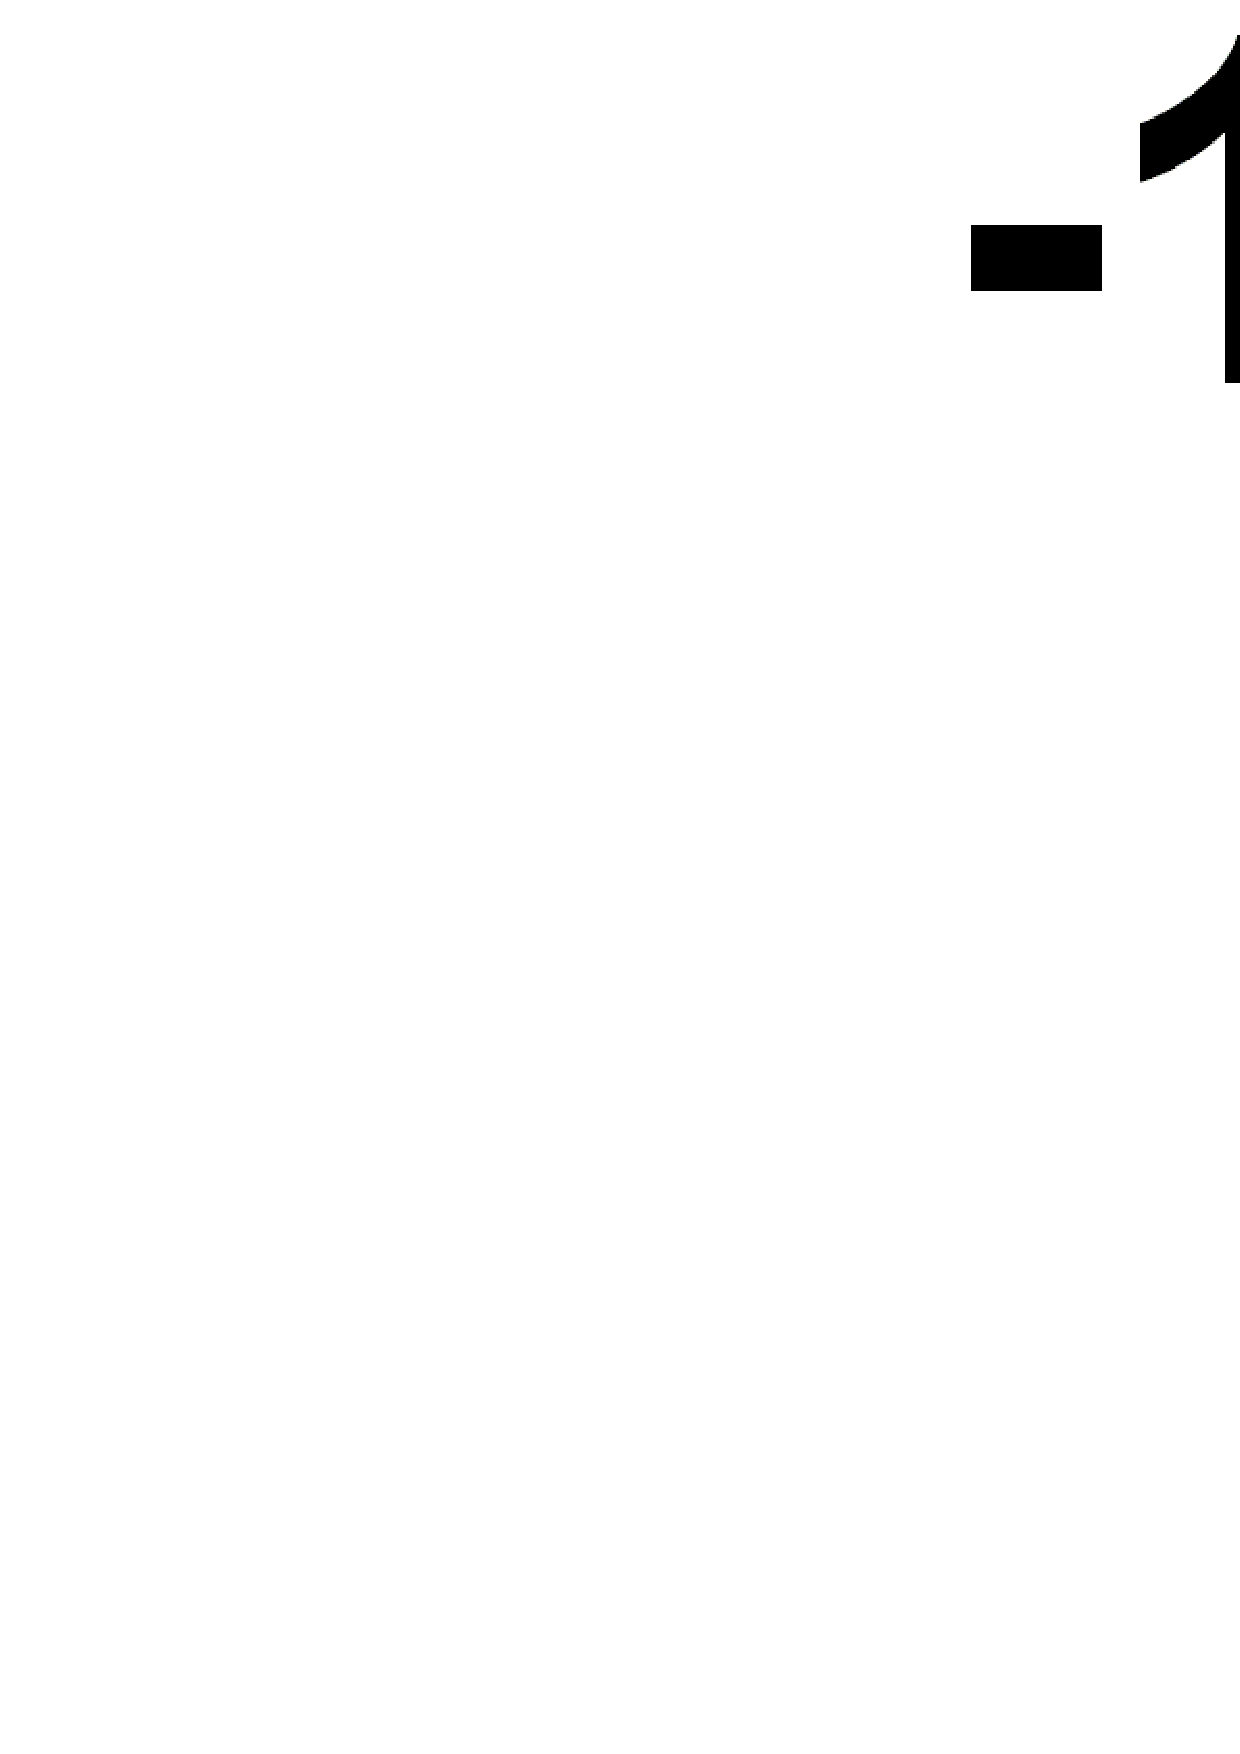
\includegraphics[width=0.45\textwidth]{olikhFig5}%
\caption{\label{fig_Erda}
Simulated dependencies of AI changes of coupling parameter on the vibration amplitudes.
Axis $|u_\mathtt{D}+u_\mathtt{A}|$ corresponds to $\delta=0^\circ$ case, whereas axis $|u_\mathtt{D}+u_\mathtt{A}|$ corresponds to $\delta=180^\circ$ case.
The parameters are set to $a_0=3.23$~nm, 
$r_{in}=5$~nm (open marks), $15$~nm (semi--filled marks), and $25$~nm (filled marks),
$\varphi=0^\circ$ (circles), $90^\circ$ (squares).
Triangles correspond to mean $\varepsilon_{\mathtt{RDA}}$ value for $[0^\circ\div 180^\circ]$ $\varphi$ range.
}%
\end{figure}

$\varepsilon_{\sigma}$ depend on oscillation amplitudes with a similar features and 
does not depend on $\varphi$: 
\begin{equation}
\label{eqEpsSig}
\varepsilon_{\sigma}=(u_\mathtt{D}\pm u_\mathtt{A})^2/2\,r_{in}^2\,,
\end{equation}
where``$+$'' and ``$-$'' correspond to $\delta=180^\circ$ and $\delta=0^\circ$ respectively.

Before analysing, it is worth keeping in mind, that 
CLDR current flows locally in the locations of extended defects\cite{CDLR:JAP,CDLR:SSP}.
On the other hand, dislocations are often situated in the SCR region perpendicularly to $p-n$ junction plane 
and investigated samples are not exception (see Section~\ref{Rsh}).
If CDLR in the dislocation locations is assumed, then dislocations with edge component would influence on pair spatial orientation.
Thus axis of donor--acceptor pair with $(\Delta\Omega_d^\mathtt{D}\cdot\Delta\Omega_d^\mathtt{A}>0)$  should be predominantly situated parallel to a dislocation line,
whereas pair of coupled defects with $(\Delta\Omega_d^\mathtt{D}\cdot\Delta\Omega_d^\mathtt{A}<0)$ should be normal.
As AW displacement is parallel to the $p-n$ junction plane,
the most excited curiosity variants are following:


%To limit concerned variant, the simple geometry would be under consideration.
%According to \cite{CDLR:JAP,CDLR:SSP}, CLDR current flows locally in the locations of extended defects,
%where a poind defect concentration is increased essentially and donor and acceptor defects can to couple to each other.
%On the other hand, dislocations are often situated in the SCR region perpendicularly to $p-n$ junction plane --- see Section~\ref{Rsh} for details.
%If CDLR in the locations of dislocation is assumed then dislocations with edge component influence on pair spatial orientation.
%Thus axes of donor--acceptor pair with $\Delta\Omega_d^\mathtt{D}\cdot\Delta\Omega_d^\mathtt{A}>0$  should be predominantly situated parallel to a dislocation line,
%whereas one of coupled defects with $\Delta\Omega_d^\mathtt{D}\cdot\Delta\Omega_d^\mathtt{A}>0$ should be normal.
%Keeping in mind, that AW displacement is parallel to the $p-n$ junction plane,
%the most excited curiosity variants are following:

\noindent  $\delta=0^\circ$, $\varphi=90^\circ$ ($\Delta\Omega_d^\mathtt{D}\cdot\Delta\Omega_d^\mathtt{A}>0$ case);

\noindent  $\delta=180^\circ$, $\varphi\in[0^\circ\div 180^\circ]$ ($\Delta\Omega_d^\mathtt{D}\cdot\Delta\Omega_d^\mathtt{A}<0$ case).

\noindent
In other words, all curves in Fig.~(\ref{fig_Erda}) can be realized if defect volume relaxation of donor--like defect opposites in sign to acceptor--like defect one.
And only squares have to be under consideration in $\Delta\Omega_d^\mathtt{D}\cdot\Delta\Omega_d^\mathtt{A}>0$ case.

In our opinion, taking into account experimental results and suggested model estimation:

\noindent
(i)~$E_{\tau g}$ and $T_{\mathrm{id}}$ are mainly determine by couple component energy levels.
The alteration of $E_{\tau g}$ and $T_{\mathrm{id}}$ for nSC, g6SC, and g7SC in comparison with iSC testifies to change of defect (donor, acceptor, or both),
which take part in CDLR, after irradiation.
And g6SC defect is coincident to g6SC defect and differs from neutron--irradiated sample defect.

\noindent
(ii)~$\varepsilon_{\tau g}$ and  $\Delta n_{\mathrm{id}}$ is caused by donor--acceptor distance change, which  
comes under USL condition, 
results in $\varepsilon_{\sigma}$ and $\varepsilon_{\mathtt{RDA}}$,
and increases with $W_{\mathtt{US}}$.

\noindent
(iii)~Acoustically induced $E_{\tau g}$ (and $T_{\mathrm{id}}$) modification, which is observed in g6SC, and g7SC only,
testifies a rebuilding of  $\gamma$--induced RD.
I.e., $\gamma$--induced RD is configurationally bistable (or metastable) and transform from ground state to another under US action.
Similar AI defect variations were also reported previously\cite{Wosinski,Ostapenko1994,Olikh2009Sem,YOlikhTPL2011}.

\noindent
(iv)~$\varepsilon_{\sigma}$ sign is immutable -- see Eq.~(\ref{eqEpsSig}), 
whereas $\varepsilon_{\mathtt{RDA}}$ sign can vary for pair with opposite relaxation volume component.
Therefore $\Delta n_{\mathrm{id}}$ and $\varepsilon_{\tau g}$ sign change is evidence of transformation
from $(\Delta\Omega_d^\mathtt{D}\cdot\Delta\Omega_d^\mathtt{A}>0)$  case to
$(\Delta\Omega_d^\mathtt{D}\cdot\Delta\Omega_d^\mathtt{A}<0)$ case after irradiation.
Transformation direction is confirmed by rise US influence efficiency in irradiated samples.
Really, in the $(\Delta\Omega_d^\mathtt{D}\cdot\Delta\Omega_d^\mathtt{A}<0)$ case the US efficiency is determined by sum of pair component displacements,
whereas in the contrary case  --- by difference.
Conceivably, both donor and acceptor are interstitial--type at non--irradiated sample, and one of pair component is vacancy--type at irradiated samples.
The defect configuration are discussed below, in Section~\ref{DefectType}.


\subsection{Quasi--neutral region\label{Base}}

Following the empirical relation proposed by Ref. 25, we assume

Some findings are shown in  Fig.~(\ref{fig_Model}).


A remarkable coupling between the
defects occurs if their density becomes so high that their
wave functions overlap. This is indeed the case in local shunt
areas: oxidized surfaces may already show a density of
defect states of about 1012
cm–2
, corresponding to a mean
distance between the defects of 10 nm.




Fig. 4 shows the  series resistance  over the explored temperature range.

\subsection{Defect type speculation\label{DefectType}}

\subsection{Shunt resistance\label{Rsh}}


\section{Conclusion}
In this work, 16 methods were implemented to extract the physical parameters of Schottky diodes.
To do so, experimental and synthetic $I$--$V$ data were used.
It has been analyzed the dependences of extraction accuracy of series resistance, barrier height and ideality factor on the parameters value and on the noise level of the $I$--$V$ curve.
It has been shown that the use of Lambert function for numerical calculation allows to reduce both the determination error value and the number of accuracy influencing factor; whereas the running time increases.
It has been examined the adaptive procedure, which provide selection of the $I$--$V$ data range for an auxiliary function construction taking into account the deviation of calculated curve and curve under investigation.
This procedure find out to improve the accuracy of analytical Gromov method, especially in the case of low noise level data.
In consideration of evolutionary algorithms, the MABC method is favorable over the DE, the PSO and the TLBO due to the minimal running time.
The most reliable and preferred methods seem to be evolutionary algorithms (specifically the MABC), Gromov method with adaptive procedure and Lee method.
The first one is reasonable in the case of
a small $R_s$ value (a few ohms) or a large $I_s$ value (high temperature).

Thus, ultrasound can be an effective tool for controlling silicon structure characteristics.

\bibliography{olikh}



\end{document}

